If $|\sin(z)| \leq 1$ and $z = x + iy$ and by
		            definition of $|\sin(z)|$ we have

		            \begin{equation*}|\sin~z|=\left|\frac{1}{2i}(e^{iz}-e^{-iz})\right| \leq
			            1\end{equation*}
		            Now, we can write $e^{iz} - e^{-iz}$ as
		            $e^{i(x+iy)} -
			            e^{-i(x+iy)} = e^{ix-y} - e^{-ix+y} =
			            e^{ix}e^{-y} - e^{-ix}e^{y}$ And using
		            Euler's
		            formula

		            \begin{equation*}
			            e^{ix} = \cos(x) + i\sin(x) \quad
			            \text{and}
			            \quad
			            e^{-ix} = \cos(x) - i\sin(x)
		            \end{equation*}

		            Therefore, we have

		            \begin{equation*}
			            |\sin~z|=\left|\frac{1}{2i}((\cos(x) +
			            i\sin(x))e^{-y} - (\cos(x) -
			            i\sin(x))e^{y})\right|
		            \end{equation*}

		            \begin{equation*}
			            |\sin~z|=\left|\frac{1}{2i}(\cos(x)e^{-y} +
			            i\sin(x)e^{-y} - \cos(x)e^{y} +
			            i\sin(x)e^{y})\right|
		            \end{equation*}

		            Since $1/i = -i$ this is the same as

		            \begin{equation*}
			            |\sin~z|=\left|\frac{1}{2}(i\cos(x)(e^{y}-e^{-y})
			            + \sin(x)(e^{-y} + e^{y}))\right|
		            \end{equation*}

		            And finally

		            \begin{equation*}
			            |\sin~z|=\left|(\sin(x)\cosh(y) +
			            i\cos(x)\sinh(y))\right| =
			            \sqrt{\sin^2(x)\cosh^2(y) +
				            \cos^2(x)\sinh^2(y)}
			            \leq 1
		            \end{equation*}

		            We can simplify this if we square both sides as the
		            RHS
		            is invariant. Now, we can use
		            \begin{align*}
			            (\sin(x)\cosh(y))^{2}+(\cos(x)\sinh(y))^{2}
			             &
			            =\sin^{2}(x)(1+\sinh^{2}(y))+\cos^{2}(x)~\sinh^{2}(y) \\
			             &
			            =\sin^{2}(x)+(\sin^{2}(x)+\cos^{2}(x))\sinh^{2}(y)    \\
			             & =\sin^{2}(x)+\sinh^{2}(y)
			            \\
		            \end{align*}

		            Therefore, we are looking at the complex numbers $z
			            = x
			            + iy$ such that
		            \begin{equation}\sin^{2}(x)+\sinh^{2}(y) \leq
			            1\end{equation}

		            The region described by this inequality can be
		            visualized in Figure~\ref{fig:1a}.
		            \begin{figure}[h]
			            \centering

			            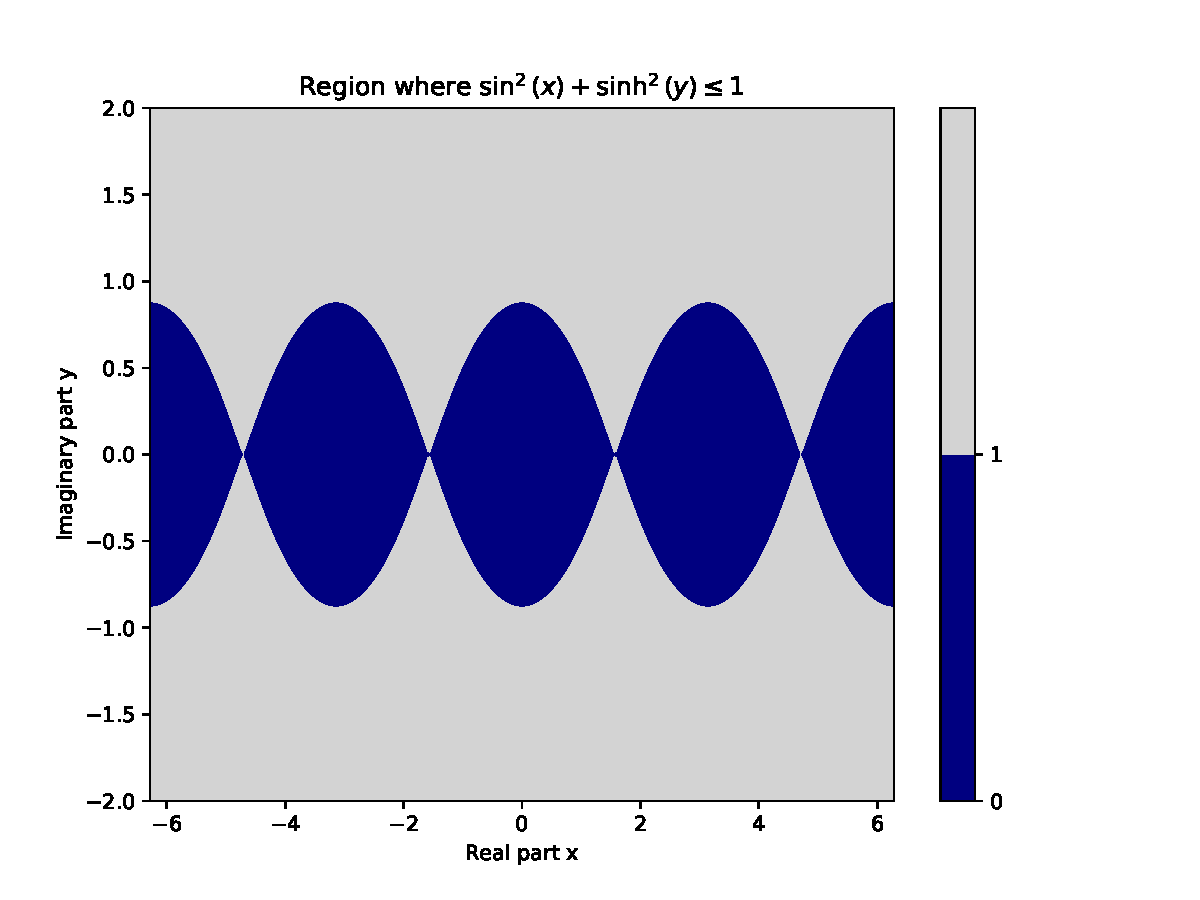
\includegraphics[width=0.5\textwidth]{sinz.pdf}
			            \caption{The region described by the
				            inequality
				            $\sin^{2}(x)+\sinh^{2}(y) \leq 1$}
			            \label{fig:1a}
		            \end{figure}